\documentclass{article}

% ─────────────────────────── PACKAGES ────────────────────────────
\usepackage{times}
\usepackage{geometry}
\geometry{a4paper,left=0.6cm,right=0.7cm,top=1cm,bottom=1cm,columnsep=0.8cm}

\usepackage{fontawesome}
\usepackage[hidelinks]{hyperref}
\usepackage{paracol}
\usepackage{tikz}
\usepackage{tabularx}
\usepackage{xcolor}
\usepackage{enumitem}


\definecolor{maincolor}{HTML}{ffffff}
\definecolor{seccolor}{HTML}{0b1f3b}
\definecolor{gray}{HTML}{8c94a9}
\definecolor{sidetext}{HTML}{59cee5}
\definecolor{Green}{HTML}{2caf00}
\definecolor{lightgray}{HTML}{D3D3D3}
%\definecolor{maincolor}{HTML}{2AAEE7}

\newcolumntype{Y}{>{\RaggedRight\arraybackslash}X}
\setlist[itemize]{itemsep=-2pt,topsep=0pt,leftmargin=*}
\renewcommand{\labelitemi}{\textcolor{black}{\footnotesize$\bullet$}}
%
\setlength{\parindent}{0pt}

% titre de section
\newcommand{\cvsection}[1]{%
  \par\bigskip
  \begin{tabular}{@{}p{\linewidth}}
  \textbf{\Large #1}\\[3pt]\hline
  \end{tabular}\medskip}

\newcommand*{\ClipSep}{0.4cm}

% ─────────────────────────── DOCUMENT ────────────────────────────
\begin{document}\pagestyle{empty}
\columnratio{0.7}\begin{paracol}{2}

%%%%%%%%%%%%%%%%%%%%%%%%%%%%%%%%%%%%%%%%%%%%%%%%%%%%%%%%%%%%%%%%%%%
% Colonne gauche (70 %)
%%%%%%%%%%%%%%%%%%%%%%%%%%%%%%%%%%%%%%%%%%%%%%%%%%%%%%%%%%%%%%%%%%%

{\LARGE\textbf{Judikael Mourouvin}}

\bigskip
{\color{sidetext}\Large\textbf{Technicien informatique et marketing digital}}

\medskip
\begin{tabular}{@{}cp{0.4\linewidth}cp{0.4\linewidth}}
  \color{sidetext}\faEnvelope & \href{mailto:jkmou971@gmail.com}{jkmou971@gmail.com} &
  \color{sidetext}\faMapMarker & Route de Cocoyer\;97190 Gosier\\[6pt]
  \color{sidetext}\faPhone & \href{tel:+590 0690 91 14 48}{+590 0690 91 14 48} &
  \color{sidetext}\faLinkedin & \href{}{}
\end{tabular}

\cvsection{EXPERIENCE}

\colorbox{maincolor}{%
  \begin{minipage}{\linewidth}
    \textbf{Alternant en Marketing Digital} \\ Mairie du Gosier – DSI \\ 2023-2024
    \begin{itemize}
      \item Coordonné des projets numériques pour moderniser les services municipaux. \item Analysé les besoins des agents puis déployé des solutions adaptées. \item Assuré le support et la formation des utilisateurs tout en soutenant la stratégie digitale.
    \end{itemize}
  \end{minipage}}

\vspace{3mm}


\colorbox{maincolor}{%
  \begin{minipage}{\linewidth}
    \textbf{Animateur de la zone informatique} \\ Pôle Emploi, Gosier \\ 2022-2023
    \begin{itemize}
      \item Fournit un support technique quotidien aux demandeurs d’emploi et conseillers. \item Installé, configuré et entretenu les postes de travail de l’espace numérique. \item Diagnostiqué et résolu les incidents afin de garantir la disponibilité des équipements.
    \end{itemize}
  \end{minipage}}

\vspace{3mm}


\colorbox{maincolor}{%
  \begin{minipage}{\linewidth}
    \textbf{Stagiaire Informaticien} \\ Numerika, Baie-Mahault \\ 2020-2021
    \begin{itemize}
      \item Configuré et maintenu postes et périphériques dans le parc informatique. \item Offert un support utilisateur de premier niveau pour les problèmes courants. \item Participé au déploiement d’équipements pour améliorer la productivité interne.
    \end{itemize}
  \end{minipage}}      %← généré dynamiquement (blocs colorbox)

\cvsection{EDUCATION}

    \begin{tabularx}{\linewidth}{@{}c X@{}}
    \textcolor{sidetext}{\faGraduationCap} &
    \textbf{Bachelor Marketing Digital} \\
    & CFA IUTS \\
    & \begin{itemize}[leftmargin=*]
  \item Stratégies de communication numérique et gestion de contenu. \item Mise en œuvre de campagnes SEO/SEA et analyse de performance. \item Pilotage de projets digitaux et reporting des indicateurs clés.
\end{itemize} \\
    & \textit{2023-2024}
    \end{tabularx}
    

\vspace{3mm}


    \begin{tabularx}{\linewidth}{@{}c X@{}}
    \textcolor{sidetext}{\faGraduationCap} &
    \textbf{BTS Système Numérique option Informatique et Réseaux} \\
    & Lycée de Chevalier Saint-Georges, Abymes \\
    & \begin{itemize}[leftmargin=*]
  \item Conception et administration de réseaux locaux et étendus. \item Maintenance matérielle et logicielle des systèmes informatiques. \item Développement et déploiement de solutions embarquées.
\end{itemize} \\
    & \textit{2019-2021}
    \end{tabularx}
              %← idem



%%%%%%%%%%%%%%%%%%%%%%%%%%%%%%%%%%%%%%%%%%%%%%%%%%%%%%%%%%%%%%%%%%%
% Colonne droite (30 %)
%%%%%%%%%%%%%%%%%%%%%%%%%%%%%%%%%%%%%%%%%%%%%%%%%%%%%%%%%%%%%%%%%%%
\switchcolumn
\centering
\begin{tikzpicture}
  \clip (0,0) circle (1.5cm) node[anchor=center]
        {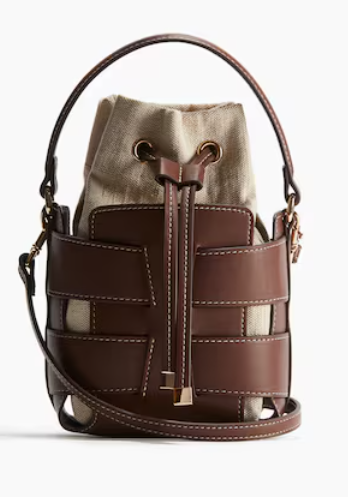
\includegraphics[width=3cm]{5069bbc638714580b60c3ca52c73a2e1.png}};
\end{tikzpicture}


\cvsection{SUMMARY}
Passionné par l’informatique et le marketing digital, je maîtrise la configuration de postes, la maintenance matérielle et la résolution d’incidents. Mon année d’alternance à la DSI de la Mairie du Gosier m’a permis de gérer des projets numériques et d’accompagner les utilisateurs. Rigoureux et orienté résultats, je souhaite désormais évoluer à plein temps pour contribuer au succès de vos initiatives digitales. Mon objectif : mettre mes compétences techniques et mon sens du service au profit de votre organisation.

\cvsection{SKILLS}
\begin{itemize}[leftmargin=*]
\item Réseaux
\item Support
\item Maintenance
\item Marketing
\item Digital
\item Configuration
\item Diagnostic\end{itemize}

\cvsection{LANGUAGES}
\begin{itemize}[leftmargin=*]
\item English - \textcolor{gray}{}
\item Espagnol - \textcolor{gray}{}\end{itemize}

\cvsection{INTERESTS}
\begin{itemize}[leftmargin=*]
\item Lecture \& veille technologique
\item Randonnée / sports outdoor
\item Voyages \& découverte culturelle
\end{itemize}

\end{paracol}
\end{document}
